% ============================================================
% 培优专题一：几何辅助线八大技巧（完整版）
% 编译命令：xelatex -interaction=nonstopmode 培优专题1_几何辅助线八大技巧.tex
% ============================================================
\documentclass[12pt, a4paper]{ctexart}
\usepackage[margin=2.2cm]{geometry}
\usepackage{amsmath, amssymb}
\usepackage{enumitem}
\usepackage{tcolorbox}
\usepackage{booktabs}
\usepackage{array}
\usepackage{fancyhdr}
\usepackage{xcolor}
\usepackage{tikz}
\usepackage{hyperref}
\usepackage{graphicx}
\usepackage{multirow}
\usepackage{pgfplots}
\usepackage{amsthm}
\pgfplotsset{compat=1.18}
\usetikzlibrary{calc, angles, quotes, patterns, decorations.markings, intersections}

% 颜色定义
\definecolor{mainblue}{RGB}{41, 98, 168}
\definecolor{lightblue}{RGB}{230, 240, 255}
\definecolor{tipgreen}{RGB}{34, 139, 87}
\definecolor{lightgreen}{RGB}{235, 250, 240}
\definecolor{warnred}{RGB}{200, 50, 50}
\definecolor{lightred}{RGB}{255, 240, 240}
\definecolor{examorange}{RGB}{210, 120, 20}
\definecolor{lightorange}{RGB}{255, 248, 235}
\definecolor{apppurple}{RGB}{120, 60, 170}
\definecolor{lightpurple}{RGB}{245, 238, 255}
\definecolor{dashgray}{RGB}{120, 120, 120}

% 页眉页脚
\pagestyle{fancy}
\fancyhf{}
\fancyhead[L]{\small\textcolor{mainblue}{\textbf{初中数学培优 \(\cdot\) 几何辅助线}}}
\fancyhead[R]{\small\textcolor{mainblue}{培优专题一}}
\fancyfoot[C]{\small —\ \thepage\ —}
\renewcommand{\headrulewidth}{0.6pt}
\renewcommand{\headrule}{\hbox to\headwidth{\color{mainblue}\leaders\hrule height \headrulewidth\hfill}}
\renewcommand{\footrulewidth}{0pt}

% tcolorbox 样式
\newtcolorbox{knowledgebox}[1][]{%
  colback=lightblue, colframe=mainblue,
  fonttitle=\bfseries\large, title=#1,
  arc=3mm, boxrule=0.8pt,
  left=8pt, right=8pt, top=6pt, bottom=6pt
}

\newtcolorbox{tipbox}[1][]{%
  colback=lightgreen, colframe=tipgreen,
  fonttitle=\bfseries, title=#1,
  arc=2mm, boxrule=0.6pt,
  left=6pt, right=6pt, top=4pt, bottom=4pt
}

\newtcolorbox{warnbox}[1][]{%
  colback=lightred, colframe=warnred,
  fonttitle=\bfseries, title=#1,
  arc=2mm, boxrule=0.6pt,
  left=6pt, right=6pt, top=4pt, bottom=4pt
}

\newtcolorbox{examplebox}[1][]{%
  colback=lightorange, colframe=examorange,
  fonttitle=\bfseries, title=#1,
  arc=3mm, boxrule=0.8pt,
  left=8pt, right=8pt, top=6pt, bottom=6pt
}

\newtcolorbox{appbox}[1][]{%
  colback=lightpurple, colframe=apppurple,
  fonttitle=\bfseries, title=#1,
  arc=3mm, boxrule=0.8pt,
  left=8pt, right=8pt, top=6pt, bottom=6pt
}

\newtcolorbox{exerbox}[1][]{%
  colback=white, colframe=dashgray,
  fonttitle=\bfseries, title=#1,
  arc=2mm, boxrule=0.6pt,
  left=8pt, right=8pt, top=4pt, bottom=4pt
}

\setCJKmainfont{Hiragino Sans GB}
\setCJKsansfont{Heiti SC}

\begin{document}

% ============ 标题页 ============
\begin{center}
{\Huge\bfseries\textcolor{mainblue}{几何辅助线八大技巧}}\\[12pt]
{\Large\textcolor{gray}{培优专题讲义}}\\[8pt]
\rule{0.6\textwidth}{1pt}\\[8pt]
{\normalsize 适用：初中数学培优\quad |\quad 难度：中考压轴 \(\sim\) 竞赛入门}
\end{center}
\vspace{6pt}

\begin{knowledgebox}[写在前面]
几何辅助线是平面几何的核心技能。很多同学面对几何题"想不到辅助线"，其实辅助线并非凭空而来，而是有章可循的。本讲义系统总结初中阶段最常用的八大辅助线技巧，每种技巧配有原理说明、经典例题和方法总结。掌握这些技巧，中考几何压轴题和竞赛入门题将不再困难。

\medskip
\noindent\textbf{学习建议：}
\begin{enumerate}[leftmargin=2em]
  \item 先理解每种技巧的\textbf{原理}和\textbf{适用场景}；
  \item 认真研读例题的\textbf{解题思路}，注意辅助线是"怎么想到的"；
  \item 独立完成综合练习，对照参考答案查漏补缺；
  \item 反复练习，形成"看到条件 \(\to\) 联想辅助线"的条件反射。
\end{enumerate}
\end{knowledgebox}

\vspace{4pt}

% ============================================================
%  技巧一：倍长中线法
% ============================================================
\section*{\textcolor{mainblue}{技巧一：倍长中线法}}

\begin{knowledgebox}[什么是倍长中线法？]
\textbf{核心原理：}将三角形的中线延长一倍，连接端点，构造一对全等三角形，从而实现线段或角度的转移。

\medskip
\noindent\textbf{适用场景：}
\begin{itemize}[leftmargin=1.5em]
  \item 题目中出现\textbf{中线}（或中点条件）；
  \item 需要证明线段的\textbf{不等关系}（如 \(AB + AC > 2AD\)）；
  \item 需要证明线段\textbf{相等}或直线\textbf{平行}；
  \item 需要将分散的线段集中到一个三角形中。
\end{itemize}

\medskip
\noindent\textbf{操作方法：}

如图，\(\triangle ABC\) 中，\(AD\) 是 \(BC\) 边上的中线。延长 \(AD\) 至 \(E\)，使 \(DE = AD\)，连接 \(BE\)。

\begin{center}
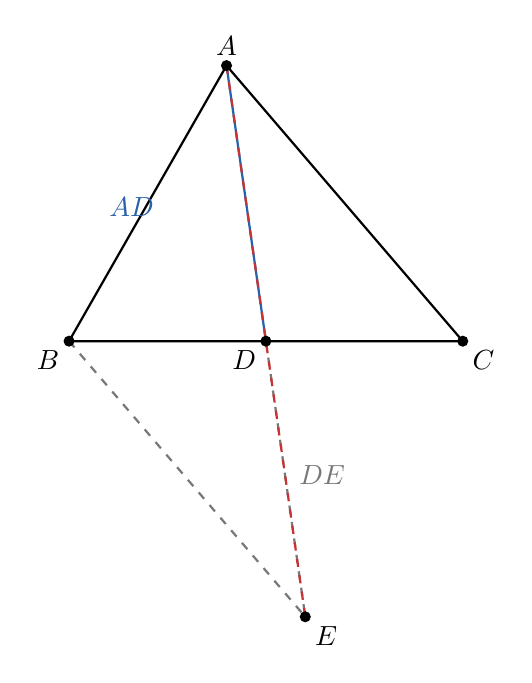
\begin{tikzpicture}[scale=1.0]
  \coordinate (A) at (2, 3.5);
  \coordinate (B) at (0, 0);
  \coordinate (C) at (5, 0);
  \coordinate (D) at (2.5, 0);
  \coordinate (E) at (3, -3.5);
  \draw[thick] (A)--(B)--(C)--cycle;
  \draw[thick, mainblue] (A)--(D);
  \draw[thick, dashed, dashgray] (D)--(E);
  \draw[thick, dashed, dashgray] (B)--(E);
  \draw[thick, dashed, warnred] (A)--(E);
  \fill (D) circle (2pt) node[below left] {\(D\)};
  \fill (A) circle (2pt) node[above] {\(A\)};
  \fill (B) circle (2pt) node[below left] {\(B\)};
  \fill (C) circle (2pt) node[below right] {\(C\)};
  \fill (E) circle (2pt) node[below right] {\(E\)};
  \node[mainblue, left] at (1.2, 1.7) {\(AD\)};
  \node[dashgray, right] at (2.8, -1.7) {\(DE\)};
\end{tikzpicture}
\end{center}

\(\because BD = CD\)，\(AD = DE\)，\(\angle ADB = \angle EDC\)（对顶角），

\(\therefore \triangle ADB \cong \triangle EDC\)（SAS），

\(\therefore AB = EC\)，\(\angle BAD = \angle CED\)。

这样就把 \(AB\) 转移到了 \(CE\) 的位置，\(AB\)、\(AC\)、\(2AD\) 集中在 \(\triangle ACE\) 中。
\end{knowledgebox}

% --- 例题 1-1 ---
\begin{examplebox}[【例题 1-1】倍长中线证不等式]
\textbf{已知：}在 \(\triangle ABC\) 中，\(AD\) 是 \(BC\) 边上的中线。

\textbf{求证：}\(AB + AC > 2AD\)。
\end{examplebox}

\noindent\textbf{证明：}

延长 \(AD\) 至 \(E\)，使 \(DE = AD\)，连接 \(BE\)。

\begin{center}
\begin{tikzpicture}[scale=1.1]
  \coordinate (A) at (2, 3.5);
  \coordinate (B) at (0, 0);
  \coordinate (C) at (5, 0);
  \coordinate (D) at (2.5, 0);
  \coordinate (E) at (3, -3.5);
  \draw[thick] (A)--(B)--(C)--cycle;
  \draw[thick, mainblue] (A)--(D);
  \draw[thick, dashed, dashgray] (D)--(E);
  \draw[thick, dashed, dashgray] (B)--(E);
  \draw[thick, warnred, dashed] (A)--(E);
  \fill (D) circle (2pt) node[below left] {\(D\)};
  \fill (A) circle (2pt) node[above] {\(A\)};
  \fill (B) circle (2pt) node[below left] {\(B\)};
  \fill (C) circle (2pt) node[below right] {\(C\)};
  \fill (E) circle (2pt) node[below right] {\(E\)};
\end{tikzpicture}
\end{center}

在 \(\triangle ADB\) 和 \(\triangle EDC\) 中：
\[BD = DC, \quad AD = DE, \quad \angle ADB = \angle EDC\]

\(\therefore \triangle ADB \cong \triangle EDC\)（SAS），

\(\therefore AB = EC\)。

在 \(\triangle ACE\) 中，由三角不等式：
\[AC + CE > AE\]

即 \(AC + AB > AD + DE = 2AD\)。

\(\therefore AB + AC > 2AD\)。\hfill\(\square\)

\begin{tipbox}[思路点拨]
本题的关键是：\textbf{倍长中线后，将 \(AB\) 转移到 \(CE\) 位置}，使得 \(AB\)、\(AC\)、\(2AD\) 三条线段集中在同一个 \(\triangle ACE\) 中，从而可以直接使用三角不等式。这是倍长中线法最经典的应用。
\end{tipbox}

% --- 例题 1-2 ---
\begin{examplebox}[【例题 1-2】倍长中线证比例]
\textbf{已知：}如图，在 \(\triangle ABC\) 中，\(D\) 为 \(BC\) 的中点，\(E\) 为 \(AD\) 的中点，连接 \(BE\) 并延长交 \(AC\) 于 \(F\)。

\textbf{求证：}\(AF = \dfrac{1}{2}FC\)（即 \(F\) 为 \(AC\) 的三等分点）。
\end{examplebox}

\noindent\textbf{证明：}

\begin{center}
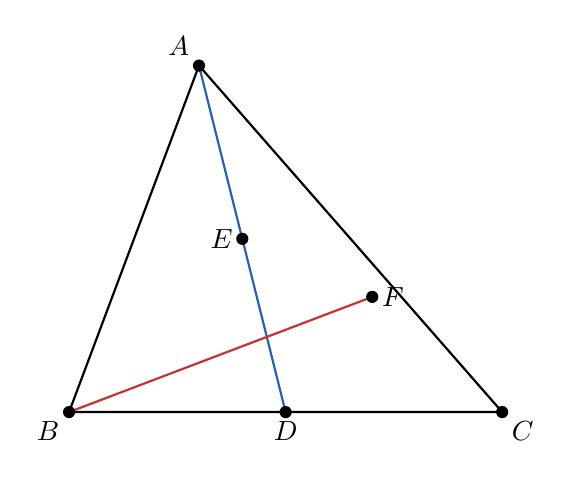
\begin{tikzpicture}[scale=1.1]
  \coordinate (A) at (1.5, 4);
  \coordinate (B) at (0, 0);
  \coordinate (C) at (5, 0);
  \coordinate (D) at (2.5, 0);
  \coordinate (E) at (2, 2);
  \coordinate (F) at (3.5, 1.33);
  \draw[thick] (A)--(B)--(C)--cycle;
  \draw[thick, mainblue] (A)--(D);
  \draw[thick, warnred] (B)--(F);
  \fill (A) circle (2pt) node[above left] {\(A\)};
  \fill (B) circle (2pt) node[below left] {\(B\)};
  \fill (C) circle (2pt) node[below right] {\(C\)};
  \fill (D) circle (2pt) node[below] {\(D\)};
  \fill (E) circle (2pt) node[left] {\(E\)};
  \fill (F) circle (2pt) node[right] {\(F\)};
\end{tikzpicture}
\end{center}

延长 \(ED\) 至 \(G\)，使 \(DG = ED\)，连接 \(CG\)。

\begin{center}
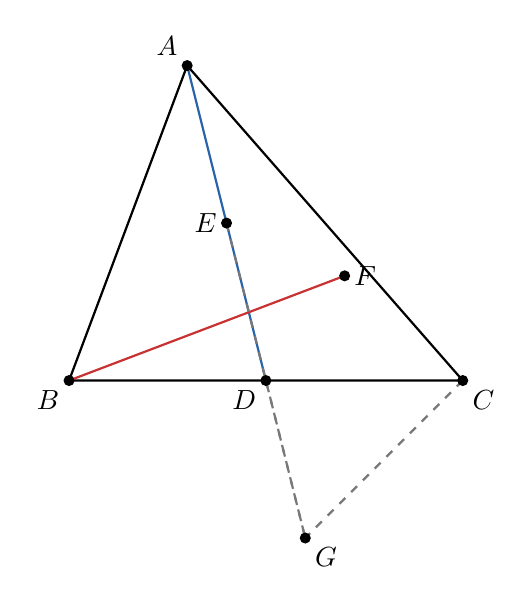
\begin{tikzpicture}[scale=1.0]
  \coordinate (A) at (1.5, 4);
  \coordinate (B) at (0, 0);
  \coordinate (C) at (5, 0);
  \coordinate (D) at (2.5, 0);
  \coordinate (E) at (2, 2);
  \coordinate (F) at (3.5, 1.33);
  \coordinate (G) at (3, -2);
  \draw[thick] (A)--(B)--(C)--cycle;
  \draw[thick, mainblue] (A)--(D);
  \draw[thick, warnred] (B)--(F);
  \draw[thick, dashed, dashgray] (D)--(G);
  \draw[thick, dashed, dashgray] (E)--(G);
  \draw[thick, dashed, dashgray] (C)--(G);
  \fill (A) circle (2pt) node[above left] {\(A\)};
  \fill (B) circle (2pt) node[below left] {\(B\)};
  \fill (C) circle (2pt) node[below right] {\(C\)};
  \fill (D) circle (2pt) node[below left] {\(D\)};
  \fill (E) circle (2pt) node[left] {\(E\)};
  \fill (F) circle (2pt) node[right] {\(F\)};
  \fill (G) circle (2pt) node[below right] {\(G\)};
\end{tikzpicture}
\end{center}

在 \(\triangle BDE\) 和 \(\triangle CDG\) 中：
\[BD = CD, \quad ED = DG, \quad \angle BDE = \angle CDG\]

\(\therefore \triangle BDE \cong \triangle CDG\)（SAS），

\(\therefore BE = CG\)，\(\angle DBE = \angle DCG\)。

\(\therefore BF \parallel CG\)（内错角相等）。

在 \(\triangle ACG\) 中，\(E\) 为 \(AD\) 的中点，\(AE = ED = DG\)，故 \(AE:EG = 1:2\)。

\(\because BF \parallel CG\)，由平行线分线段成比例定理：
\[\frac{AF}{FC} = \frac{AE}{EG} = \frac{1}{2}\]

\(\therefore AF = \dfrac{1}{2}FC\)。\hfill\(\square\)

\begin{tipbox}[方法总结]
\textbf{倍长中线法}的核心步骤：\textbf{一倍长、二连端、三全等、四转移}。遇到中点（中线）条件时，优先考虑此法。倍长法不仅用于三角形中线，任何涉及中点的线段都可以"倍长"。
\end{tipbox}

% ============================================================
%  技巧二：截长补短法
% ============================================================
\section*{\textcolor{mainblue}{技巧二：截长补短法}}

\begin{knowledgebox}[什么是截长补短法？]
\textbf{核心原理：}证明线段的\textbf{和差关系}（如 \(a = b + c\)）时，在长线段上截取等于短线段的部分（\textbf{截长}），或将短线段延长使之等于长线段（\textbf{补短}），从而将线段的和差关系转化为\textbf{线段相等}关系。

\medskip
\noindent\textbf{两种策略：}

\textbf{截长法：}欲证 \(AB = CD + EF\)，在 \(AB\) 上截取 \(AG = CD\)，只需证 \(GB = EF\)。

\textbf{补短法：}欲证 \(AB = CD + EF\)，延长 \(CD\) 至 \(H\) 使 \(DH = EF\)，只需证 \(AB = CH\)。

\medskip
\noindent\textbf{适用场景：}
\begin{itemize}[leftmargin=1.5em]
  \item 需要证明\textbf{线段的和差关系}；
  \item 角平分线条件下出现线段和差；
  \item 截长补短后能构造全等三角形。
\end{itemize}
\end{knowledgebox}

% --- 例题 2-1（截长法）---
\begin{examplebox}[【例题 2-1】截长法——角平分线与线段和差]
\textbf{已知：}在 \(\triangle ABC\) 中，\(\angle B = 2\angle C\)，\(AD\) 平分 \(\angle BAC\)，交 \(BC\) 于 \(D\)。

\textbf{求证：}\(AC = AB + BD\)。
\end{examplebox}

\noindent\textbf{证明：}（截长法）

在 \(AC\) 上截取 \(AE = AB\)，连接 \(DE\)。

\begin{center}
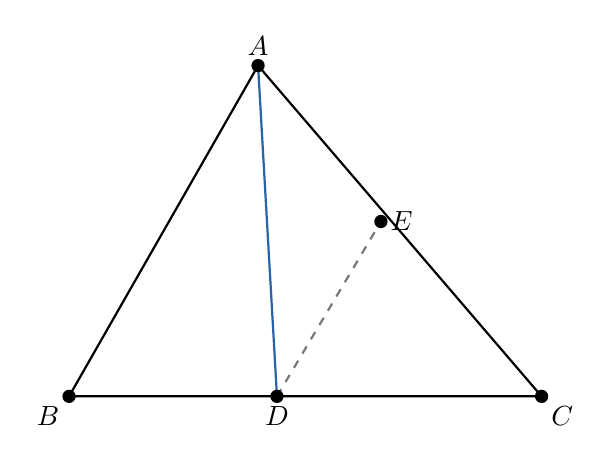
\begin{tikzpicture}[scale=1.2]
  \coordinate (A) at (2, 3.5);
  \coordinate (B) at (0, 0);
  \coordinate (C) at (5, 0);
  \coordinate (D) at (2.2, 0);
  \coordinate (E) at (3.3, 1.85);
  \draw[thick] (A)--(B)--(C)--cycle;
  \draw[thick, mainblue] (A)--(D);
  \draw[thick, dashed, dashgray] (D)--(E);
  \fill (A) circle (2pt) node[above] {\(A\)};
  \fill (B) circle (2pt) node[below left] {\(B\)};
  \fill (C) circle (2pt) node[below right] {\(C\)};
  \fill (D) circle (2pt) node[below] {\(D\)};
  \fill (E) circle (2pt) node[right] {\(E\)};
\end{tikzpicture}
\end{center}

在 \(\triangle ABD\) 和 \(\triangle AED\) 中：
\[AB = AE, \quad \angle BAD = \angle EAD, \quad AD = AD\]

\(\therefore \triangle ABD \cong \triangle AED\)（SAS），

\(\therefore BD = ED\)，\(\angle ABD = \angle AED\)。

\(\because \angle AED = \angle EDC + \angle C\)（外角定理），

\(\angle ABD = \angle AED = \angle EDC + \angle C\)。

又 \(\because \angle ABD = 2\angle C\)（已知），

\(\therefore \angle EDC + \angle C = 2\angle C\)，即 \(\angle EDC = \angle C\)。

\(\therefore \triangle EDC\) 为等腰三角形，\(ED = EC\)。

\(\therefore BD = ED = EC\)。

\(\therefore AC = AE + EC = AB + BD\)。\hfill\(\square\)

\begin{tipbox}[思路点拨]
\textbf{截长法}的关键：在长线段 \(AC\) 上截取 \(AE = AB\)，目的是构造 \(\triangle ABD \cong \triangle AED\)，从而把 \(BD\) 转移到 \(ED\) 的位置。接下来只需证 \(ED = EC\) 即可。截长后，往往能借助\textbf{角平分线}条件构造全等。
\end{tipbox}

% --- 例题 2-2（面积法建立线段关系）---
\begin{examplebox}[【例题 2-2】面积法建立倒数关系]
\textbf{已知：}在 \(\triangle ABC\) 中，\(\angle BAC = 120^\circ\)，\(AD\) 平分 \(\angle BAC\)，交 \(BC\) 于 \(D\)。

\textbf{求证：}\(\dfrac{1}{AD} = \dfrac{1}{AB} + \dfrac{1}{AC}\)。
\end{examplebox}

\noindent\textbf{证明：}

\begin{center}
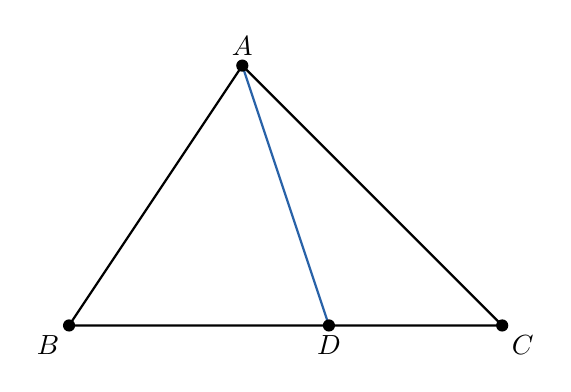
\begin{tikzpicture}[scale=1.1]
  \coordinate (A) at (2, 3);
  \coordinate (B) at (0, 0);
  \coordinate (C) at (5, 0);
  \coordinate (D) at (3, 0);
  \draw[thick] (A)--(B)--(C)--cycle;
  \draw[thick, mainblue] (A)--(D);
  \fill (A) circle (2pt) node[above] {\(A\)};
  \fill (B) circle (2pt) node[below left] {\(B\)};
  \fill (C) circle (2pt) node[below right] {\(C\)};
  \fill (D) circle (2pt) node[below] {\(D\)};
\end{tikzpicture}
\end{center}

用面积法：\(S_{\triangle ABC} = S_{\triangle ABD} + S_{\triangle ACD}\)。

\[\frac{1}{2} \cdot AB \cdot AC \cdot \sin 120^\circ = \frac{1}{2} \cdot AB \cdot AD \cdot \sin 60^\circ + \frac{1}{2} \cdot AC \cdot AD \cdot \sin 60^\circ\]

\(\because \sin 120^\circ = \sin 60^\circ\)，两边除以 \(\dfrac{1}{2} \sin 60^\circ\)：

\[AB \cdot AC = AB \cdot AD + AC \cdot AD = AD(AB + AC)\]

\[\therefore AD = \frac{AB \cdot AC}{AB + AC}\]

\[\therefore \frac{1}{AD} = \frac{AB + AC}{AB \cdot AC} = \frac{1}{AC} + \frac{1}{AB}\]

\(\therefore \dfrac{1}{AD} = \dfrac{1}{AB} + \dfrac{1}{AC}\)。\hfill\(\square\)

\begin{tipbox}[方法总结]
\textbf{截长补短法}的要诀：看到"线段和差"就想"截长或补短"。截长法——在长线段上截取；补短法——延长短线段。两种方法的目标一致：将和差关系转化为\textbf{相等关系}，然后利用\textbf{全等}或\textbf{等腰}完成证明。本题的面积法也提示我们：截长补短不是唯一手段，面积法同样能建立线段关系。
\end{tipbox}

% ============================================================
%  技巧三：角平分线辅助线
% ============================================================
\section*{\textcolor{mainblue}{技巧三：角平分线辅助线}}

\begin{knowledgebox}[角平分线辅助线的两种策略]
角平分线是非常重要的条件，围绕它可以作两类常用辅助线：

\medskip
\noindent\textbf{策略一：角平分线 + 平行线 \(\to\) 等腰三角形}

过边上一点作角平分线的平行线，可以构造等腰三角形。

\medskip
\noindent\textbf{策略二：向角两边作垂线 \(\to\) 利用"到角两边距离相等"}

角平分线上任意一点到角两边的距离相等，配合面积法使用效果极佳。
\end{knowledgebox}

% --- 例题 3-1 ---
\begin{examplebox}[【例题 3-1】角平分线 + 平行线 \(\to\) 等腰]
\textbf{已知：}如图，在 \(\triangle ABC\) 中，\(BD\) 平分 \(\angle ABC\)，\(DE \parallel BC\)，交 \(AB\) 于 \(E\)。

\textbf{求证：}\(\triangle BDE\) 为等腰三角形（即 \(BE = DE\)）。
\end{examplebox}

\noindent\textbf{证明：}

\begin{center}
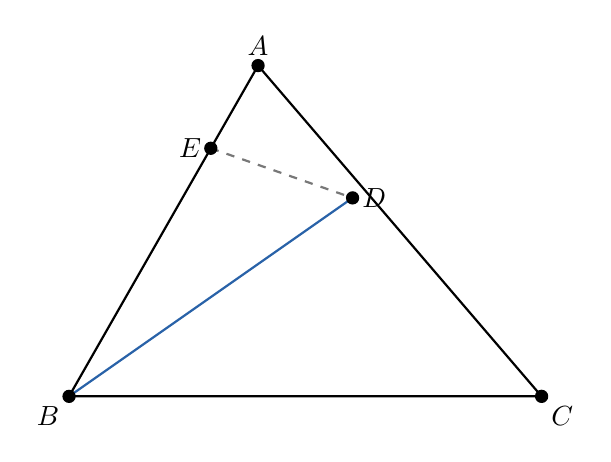
\begin{tikzpicture}[scale=1.2]
  \coordinate (A) at (2, 3.5);
  \coordinate (B) at (0, 0);
  \coordinate (C) at (5, 0);
  \coordinate (D) at (3, 2.1);
  \coordinate (E) at (1.5, 2.625);
  \draw[thick] (A)--(B)--(C)--cycle;
  \draw[thick, mainblue] (B)--(D);
  \draw[thick, dashed, dashgray] (E)--(D);
  \fill (A) circle (2pt) node[above] {\(A\)};
  \fill (B) circle (2pt) node[below left] {\(B\)};
  \fill (C) circle (2pt) node[below right] {\(C\)};
  \fill (D) circle (2pt) node[right] {\(D\)};
  \fill (E) circle (2pt) node[left] {\(E\)};
\end{tikzpicture}
\end{center}

\(\because DE \parallel BC\)，\(\therefore \angle EDB = \angle DBC\)（内错角相等）。

\(\because BD\) 平分 \(\angle ABC\)，\(\therefore \angle EBD = \angle DBC\)。

\(\therefore \angle EDB = \angle EBD\)。

\(\therefore \triangle BDE\) 为等腰三角形，\(BE = DE\)。\hfill\(\square\)

\begin{tipbox}[思路点拨]
本题体现了角平分线辅助线最常用的策略：\textbf{角平分线 + 平行线}。平行线产生的内错角与角平分线提供的等角相结合，直接得到等腰三角形。这一模式在很多复杂题目中反复出现。
\end{tipbox}

% --- 例题 3-2 ---
\begin{examplebox}[【例题 3-2】向两边作垂线——角平分线与面积]
\textbf{已知：}如图，\(\triangle ABC\) 中，\(\angle C = 90^\circ\)，\(AC = 6\)，\(BC = 8\)，\(AD\) 平分 \(\angle BAC\)。

\textbf{求：}\(BD\) 的长。
\end{examplebox}

\noindent\textbf{解：}

\begin{center}
\begin{tikzpicture}[scale=0.9]
  \coordinate (A) at (0, 6);
  \coordinate (B) at (8, 0);
  \coordinate (C) at (0, 0);
  \coordinate (D) at (4.0, 2.25);
  \draw[thick] (A)--(B)--(C)--cycle;
  \draw[thick, mainblue] (A)--(D);
  \fill (A) circle (2pt) node[above left] {\(A\)};
  \fill (B) circle (2pt) node[below right] {\(B\)};
  \fill (C) circle (2pt) node[below left] {\(C\)};
  \fill (D) circle (2pt) node[right] {\(D\)};
\end{tikzpicture}
\end{center}

过 \(D\) 作 \(DE \perp AB\) 于 \(E\)。

\(\because AD\) 平分 \(\angle BAC\)，\(\therefore DC = DE\)（角平分线上的点到两边距离相等）。

设 \(BD = x\)，则 \(CD = 8 - x\)，\(DE = DC = 8 - x\)。

在 \(Rt\triangle ABC\) 中，\(AB = \sqrt{AC^2 + BC^2} = \sqrt{36 + 64} = 10\)。

用面积法：\(S_{\triangle ABC} = S_{\triangle ABD} + S_{\triangle ACD}\)，

\[\frac{1}{2} \cdot AC \cdot BC = \frac{1}{2} \cdot AB \cdot DE + \frac{1}{2} \cdot AC \cdot CD\]

\[\frac{1}{2} \times 6 \times 8 = \frac{1}{2} \times 10 \times (8-x) + \frac{1}{2} \times 6 \times (8-x)\]

\[24 = 5(8-x) + 3(8-x) = 8(8-x)\]

\[8 - x = 3, \quad x = 5\]

\(\therefore BD = 5\)。\hfill\(\square\)

\begin{tipbox}[方法总结]
角平分线辅助线的两种核心策略：

\textbf{策略一：角平分线 + 平行线} \(\Rightarrow\) 等腰三角形。构造方法是过某点作角平分线的平行线。

\textbf{策略二：向角两边作垂线} \(\Rightarrow\) 利用"角平分线上的点到两边距离相等"，配合面积法解题。

看到角平分线，优先联想这两种辅助线。
\end{tipbox}

% ============================================================
%  技巧四：构造中位线
% ============================================================
\section*{\textcolor{mainblue}{技巧四：构造中位线}}

\begin{knowledgebox}[什么是中位线？]
\textbf{三角形中位线定理：}三角形的中位线平行于第三边，且等于第三边的一半。

\medskip
\noindent\textbf{构造中位线的思路：}
\begin{itemize}[leftmargin=1.5em]
  \item 题目中有\textbf{两个中点}（或一个中点 + 一个平行条件）；
  \item 需要证明\textbf{平行}或线段的\textbf{倍半关系}；
  \item 连接中点构成中位线，或取边的中点"凑出"中位线。
\end{itemize}

\medskip
\noindent\textbf{中点四边形：}顺次连接四边形各边中点所得的四边形是\textbf{平行四边形}。
\end{knowledgebox}

% --- 例题 4-1 ---
\begin{examplebox}[【例题 4-1】取中点构造中位线]
\textbf{已知：}如图，在 \(\triangle ABC\) 中，\(AB = AC\)，\(D\) 是 \(BC\) 的中点，\(E\) 是 \(AD\) 的中点，连接 \(CE\) 并延长交 \(AB\) 于 \(F\)。

\textbf{求证：}\(AF = \dfrac{1}{2}BF\)（即 \(F\) 三等分 \(AB\)）。
\end{examplebox}

\noindent\textbf{证明：}

\begin{center}
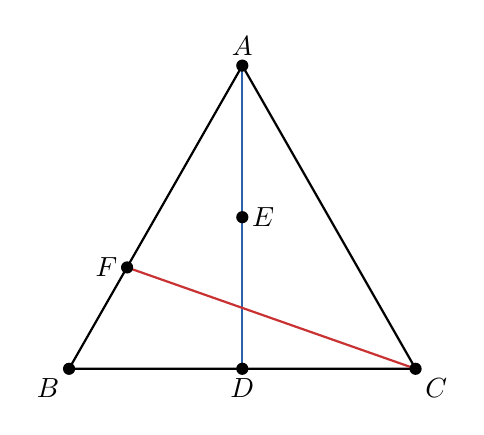
\begin{tikzpicture}[scale=1.1]
  \coordinate (A) at (2, 3.5);
  \coordinate (B) at (0, 0);
  \coordinate (C) at (4, 0);
  \coordinate (D) at (2, 0);
  \coordinate (E) at (2, 1.75);
  \coordinate (F) at (0.67, 1.17);
  \draw[thick] (A)--(B)--(C)--cycle;
  \draw[thick, mainblue] (A)--(D);
  \draw[thick, warnred] (C)--(F);
  \fill (A) circle (2pt) node[above] {\(A\)};
  \fill (B) circle (2pt) node[below left] {\(B\)};
  \fill (C) circle (2pt) node[below right] {\(C\)};
  \fill (D) circle (2pt) node[below] {\(D\)};
  \fill (E) circle (2pt) node[right] {\(E\)};
  \fill (F) circle (2pt) node[left] {\(F\)};
\end{tikzpicture}
\end{center}

取 \(BF\) 的中点 \(G\)，连接 \(DG\)。

\(\because D\) 是 \(BC\) 的中点，\(G\) 是 \(BF\) 的中点，

\(\therefore DG\) 是 \(\triangle BCF\) 的中位线，\(DG \parallel CF\)。

在 \(\triangle ADG\) 中，\(E\) 是 \(AD\) 的中点，\(EF \parallel DG\)（因为 \(CF \parallel DG\)），

\(\therefore F\) 是 \(AG\) 的中点（过三角形一边中点作另一边的平行线，必过第三边的中点）。

\(\therefore AF = FG\)。

又 \(\because G\) 是 \(BF\) 的中点，\(FG = GB\)。

\(\therefore AF = FG = GB\)，即 \(AF = \dfrac{1}{2}BF\)。\hfill\(\square\)

\begin{tipbox}[思路点拨]
本题的技巧是"取中点凑中位线"。取 \(BF\) 中点 \(G\) 后，\(DG\) 成为 \(\triangle BCF\) 的中位线，由此得到平行关系，再在 \(\triangle ADG\) 中用中位线性质完成证明。当题目涉及中点和平行/比例时，构造中位线是首选策略。
\end{tipbox}

% --- 例题 4-2 ---
\begin{examplebox}[【例题 4-2】中点四边形]
\textbf{已知：}如图，四边形 \(ABCD\) 中，\(E\)、\(F\)、\(G\)、\(H\) 分别是 \(AB\)、\(BC\)、\(CD\)、\(DA\) 的中点。

\textbf{求证：}四边形 \(EFGH\) 是平行四边形。
\end{examplebox}

\noindent\textbf{证明：}

\begin{center}
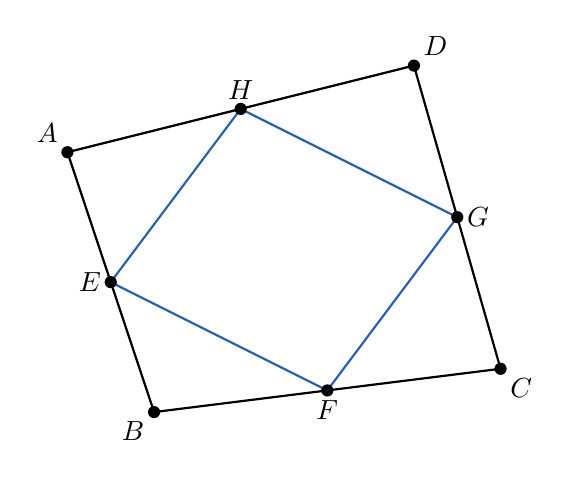
\begin{tikzpicture}[scale=1.1]
  \coordinate (A) at (0, 3);
  \coordinate (B) at (1, 0);
  \coordinate (C) at (5, 0.5);
  \coordinate (D) at (4, 4);
  \coordinate (E) at (0.5, 1.5);
  \coordinate (F) at (3, 0.25);
  \coordinate (G) at (4.5, 2.25);
  \coordinate (H) at (2, 3.5);
  \draw[thick] (A)--(B)--(C)--(D)--cycle;
  \draw[thick, mainblue] (E)--(F)--(G)--(H)--cycle;
  \fill (A) circle (2pt) node[above left] {\(A\)};
  \fill (B) circle (2pt) node[below left] {\(B\)};
  \fill (C) circle (2pt) node[below right] {\(C\)};
  \fill (D) circle (2pt) node[above right] {\(D\)};
  \fill (E) circle (2pt) node[left] {\(E\)};
  \fill (F) circle (2pt) node[below] {\(F\)};
  \fill (G) circle (2pt) node[right] {\(G\)};
  \fill (H) circle (2pt) node[above] {\(H\)};
\end{tikzpicture}
\end{center}

连接 \(AC\)。

在 \(\triangle ABC\) 中，\(E\)、\(F\) 分别是 \(AB\)、\(BC\) 的中点，

\(\therefore EF\) 是中位线，\(EF \parallel AC\) 且 \(EF = \dfrac{1}{2}AC\)。

在 \(\triangle ADC\) 中，\(H\)、\(G\) 分别是 \(DA\)、\(DC\) 的中点，

\(\therefore HG\) 是中位线，\(HG \parallel AC\) 且 \(HG = \dfrac{1}{2}AC\)。

\(\therefore EF \parallel HG\) 且 \(EF = HG\)。

\(\therefore\) 四边形 \(EFGH\) 是平行四边形（一组对边平行且相等）。\hfill\(\square\)

\begin{warnbox}[拓展思考]
如果原四边形 \(ABCD\) 是特殊四边形，中点四边形 \(EFGH\) 有什么特殊性质？
\begin{itemize}[leftmargin=1.5em]
  \item \(ABCD\) 是矩形 \(\Rightarrow\) \(EFGH\) 是\textbf{菱形}；
  \item \(ABCD\) 是菱形 \(\Rightarrow\) \(EFGH\) 是\textbf{矩形}；
  \item \(ABCD\) 是正方形 \(\Rightarrow\) \(EFGH\) 是\textbf{正方形}；
  \item \(AC \perp BD\) \(\Rightarrow\) \(EFGH\) 是\textbf{矩形}；
  \item \(AC = BD\) \(\Rightarrow\) \(EFGH\) 是\textbf{菱形}。
\end{itemize}
\end{warnbox}

\begin{tipbox}[方法总结]
\textbf{构造中位线}的关键：找到两个中点，连接它们形成中位线。如果题目只给一个中点，可以考虑\textbf{取另一个中点}来凑出中位线。中位线的两大作用：\textbf{证明平行}和\textbf{证明倍半关系}。中点四边形问题是中位线定理的直接应用。
\end{tipbox}

% ============================================================
%  技巧五：作平行线
% ============================================================
\section*{\textcolor{mainblue}{技巧五：作平行线}}

\begin{knowledgebox}[作平行线的作用]
作平行线是最通用的辅助线技巧之一，主要有两大作用：

\medskip
\noindent\textbf{作用一：转移角度}

平行线产生的\textbf{同位角}和\textbf{内错角}相等，可以将分散的角度集中到一处。

\medskip
\noindent\textbf{作用二：构造相似（或比例关系）}

平行线截三角形的两边，由\textbf{平行线分线段成比例}定理，可以得到线段的比例关系，进而证明线段相等或求线段长。
\end{knowledgebox}

% --- 例题 5-1 ---
\begin{examplebox}[【例题 5-1】平行线转移角度——拐角模型]
\textbf{已知：}如图，\(AB \parallel CD\)，\(\angle B = 35^\circ\)，\(\angle D = 25^\circ\)。

\textbf{求：}\(\angle BED\) 的度数。
\end{examplebox}

\noindent\textbf{解：}

过 \(E\) 作 \(EF \parallel AB\)（则 \(EF \parallel CD\)）。

\begin{center}
\begin{tikzpicture}[scale=1.1]
  \coordinate (A) at (-3, 2);
  \coordinate (B1) at (3, 2);
  \coordinate (C) at (-3, -2);
  \coordinate (D1) at (3, -2);
  \coordinate (E) at (0, 0);
  \draw[thick] (A)--(B1);
  \draw[thick] (C)--(D1);
  \draw[thick, mainblue] (0.5, 2)--(E)--(1.5, -2);
  \draw[thick, dashed, dashgray] (-3, 0)--(3, 0);
  \fill (E) circle (2pt) node[below left] {\(E\)};
  \node at (0.5, 2.3) {\(B\)};
  \node at (1.5, -2.3) {\(D\)};
  \node at (-3, 2.3) {\(A\)};
  \node at (-3, -2.3) {\(C\)};
  \node[dashgray] at (3.2, 0) {\(F\)};
\end{tikzpicture}
\end{center}

\(\because EF \parallel AB\)，\(\therefore \angle BEF = \angle B = 35^\circ\)（内错角相等）。

\(\because EF \parallel CD\)，\(\therefore \angle DEF = \angle D = 25^\circ\)（内错角相等）。

\(\therefore \angle BED = \angle BEF + \angle DEF = 35^\circ + 25^\circ = 60^\circ\)。\hfill\(\square\)

\begin{tipbox}[思路点拨]
本题的关键是过拐点 \(E\) 作平行线 \(EF\)。这是一类经典模型——"拐角模型"：两条平行线之间有一个拐点，过拐点作平行线即可将角度拆分求和。结论可记忆为：\(\angle BED = \angle B + \angle D\)。
\end{tipbox}

% --- 例题 5-2 ---
\begin{examplebox}[【例题 5-2】平行线构造比例]
\textbf{已知：}如图，在 \(\triangle ABC\) 中，\(D\) 为 \(BC\) 的中点，\(E\) 在 \(AD\) 上且 \(AE = 2ED\)，连接 \(BE\) 并延长交 \(AC\) 于 \(F\)。

\textbf{求证：}\(AF = FC\)（即 \(F\) 为 \(AC\) 的中点）。
\end{examplebox}

\noindent\textbf{证明：}

过 \(A\) 作 \(AG \parallel BC\)，交 \(BF\) 延长线于 \(G\)。

\begin{center}
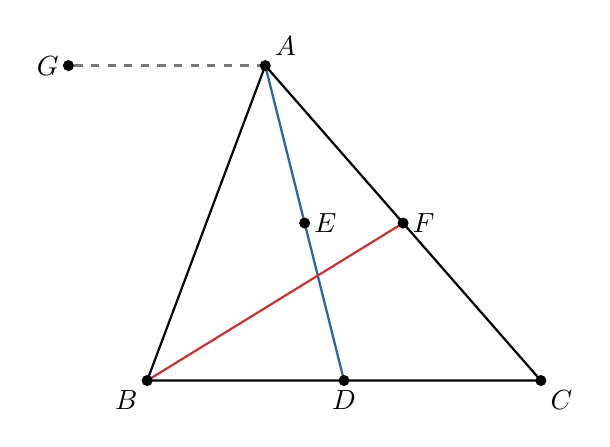
\begin{tikzpicture}[scale=1.0]
  \coordinate (A) at (1.5, 4);
  \coordinate (B) at (0, 0);
  \coordinate (C) at (5, 0);
  \coordinate (D) at (2.5, 0);
  \coordinate (E) at (2, 2);
  \coordinate (F) at (3.25, 2);
  \coordinate (G) at (-1.0, 4);
  \draw[thick] (A)--(B)--(C)--cycle;
  \draw[thick, mainblue] (A)--(D);
  \draw[thick, warnred] (B)--(F);
  \draw[thick, dashed, dashgray] (A)--(G);
  \fill (A) circle (2pt) node[above right] {\(A\)};
  \fill (B) circle (2pt) node[below left] {\(B\)};
  \fill (C) circle (2pt) node[below right] {\(C\)};
  \fill (D) circle (2pt) node[below] {\(D\)};
  \fill (E) circle (2pt) node[right] {\(E\)};
  \fill (F) circle (2pt) node[right] {\(F\)};
  \fill (G) circle (2pt) node[left] {\(G\)};
\end{tikzpicture}
\end{center}

\(\because AG \parallel BC\)，\(\therefore \triangle AEG \sim \triangle DEB\)（AA 相似），

\[\frac{AG}{BD} = \frac{AE}{ED} = \frac{2}{1}\]

\(\therefore AG = 2BD\)。

\(\because AG \parallel BC\)，\(\therefore \triangle AGF \sim \triangle CBF\)（AA 相似），

\[\frac{AF}{FC} = \frac{AG}{BC} = \frac{2BD}{BC}\]

\(\because D\) 为 \(BC\) 中点，\(BD = \dfrac{1}{2}BC\)，\(\therefore AG = 2 \cdot \dfrac{1}{2}BC = BC\)。

\[\frac{AF}{FC} = \frac{BC}{BC} = 1\]

\(\therefore AF = FC\)。\hfill\(\square\)

\begin{tipbox}[方法总结]
\textbf{作平行线}转移角度或构造比例的关键：找好"出发点"——通常是在某个顶点或分点作已知线段的平行线。平行线产生相似三角形（或比例线段），再结合已知比例条件求解。"过某点作平行线"是处理比例问题的万能工具。
\end{tipbox}

% ============================================================
%  技巧六：旋转法
% ============================================================
\section*{\textcolor{mainblue}{技巧六：旋转法}}

\begin{knowledgebox}[什么是旋转法？]
\textbf{核心原理：}将图形中的某部分绕某个点旋转一定角度（通常 \(60^\circ\)、\(90^\circ\)），构造全等三角形，从而转移线段和角度。

\medskip
\noindent\textbf{适用场景：}
\begin{itemize}[leftmargin=1.5em]
  \item 题目中有\textbf{正方形}（旋转 \(90^\circ\)）或\textbf{等边三角形}（旋转 \(60^\circ\)）；
  \item 有\textbf{共顶点的等线段}；
  \item 需要将分散的线段"旋转"到一处。
\end{itemize}

\medskip
\noindent\textbf{关键性质：}旋转前后的图形\textbf{全等}，对应线段相等，对应角相等。
\end{knowledgebox}

% --- 例题 6-1 ---
\begin{examplebox}[【例题 6-1】等边三角形中的旋转]
\textbf{已知：}如图，\(\triangle ABC\) 是等边三角形，\(P\) 是 \(\triangle ABC\) 内一点，\(PA = 3\)，\(PB = 4\)，\(PC = 5\)。

\textbf{求：}\(\angle BPC\) 的度数。
\end{examplebox}

\noindent\textbf{解：}

\begin{center}
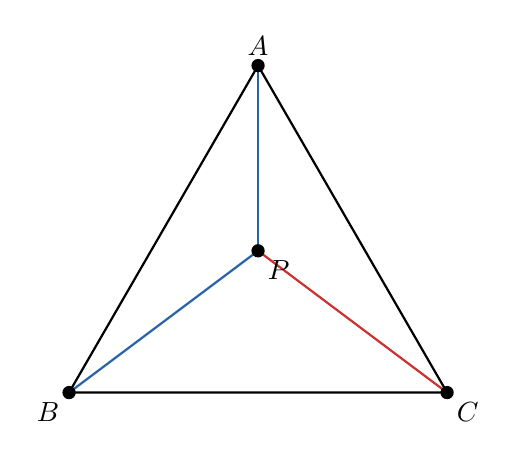
\begin{tikzpicture}[scale=1.2]
  \coordinate (A) at (2, 3.46);
  \coordinate (B) at (0, 0);
  \coordinate (C) at (4, 0);
  \coordinate (P) at (2, 1.5);
  \draw[thick] (A)--(B)--(C)--cycle;
  \draw[thick, mainblue] (P)--(A);
  \draw[thick, mainblue] (P)--(B);
  \draw[thick, warnred] (P)--(C);
  \fill (A) circle (2pt) node[above] {\(A\)};
  \fill (B) circle (2pt) node[below left] {\(B\)};
  \fill (C) circle (2pt) node[below right] {\(C\)};
  \fill (P) circle (2pt) node[below right] {\(P\)};
\end{tikzpicture}
\end{center}

将 \(\triangle ABP\) 绕点 \(B\) 顺时针旋转 \(60^\circ\)，使 \(A\) 与 \(C\) 重合。

设 \(P\) 旋转到 \(P'\)，则 \(\triangle BPP'\) 是等边三角形（\(BP = BP'\)，\(\angle PBP' = 60^\circ\)）。

\(\therefore PP' = BP = 4\)，\(CP' = AP = 3\)。

在 \(\triangle CPP'\) 中，\(CP = 5\)，\(CP' = 3\)，\(PP' = 4\)。

\(\because 3^2 + 4^2 = 9 + 16 = 25 = 5^2\)，

\(\therefore \triangle CPP'\) 是直角三角形，\(\angle CP'P = 90^\circ\)。

\(\therefore \angle BPC = \angle BPP' + \angle P'PC = 60^\circ + 90^\circ = 150^\circ\)。\hfill\(\square\)

\begin{tipbox}[思路点拨]
本题将 \(\triangle ABP\) 旋转 \(60^\circ\)，利用等边三角形的性质将三条分散的线段 \(PA\)、\(PB\)、\(PC\) 集中到 \(\triangle CPP'\) 中。发现 \(3^2 + 4^2 = 5^2\) 即可判定为直角三角形，巧妙求出角度。
\end{tipbox}

% --- 例题 6-2 ---
\begin{examplebox}[【例题 6-2】正方形中旋转 \(90^\circ\)]
\textbf{已知：}如图，正方形 \(ABCD\) 中，\(E\) 在 \(BC\) 上，\(F\) 在 \(CD\) 上，且 \(\angle EAF = 45^\circ\)。

\textbf{求证：}\(EF = BE + DF\)。
\end{examplebox}

\noindent\textbf{证明：}

\begin{center}
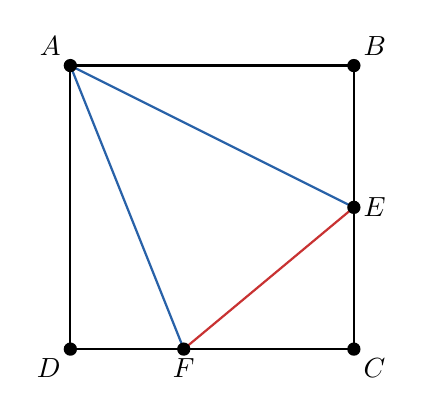
\begin{tikzpicture}[scale=1.2]
  \coordinate (A) at (0, 3);
  \coordinate (B) at (3, 3);
  \coordinate (C) at (3, 0);
  \coordinate (D) at (0, 0);
  \coordinate (E) at (3, 1.5);
  \coordinate (F) at (1.2, 0);
  \draw[thick] (A)--(B)--(C)--(D)--cycle;
  \draw[thick, mainblue] (A)--(E);
  \draw[thick, mainblue] (A)--(F);
  \draw[thick, warnred] (E)--(F);
  \fill (A) circle (2pt) node[above left] {\(A\)};
  \fill (B) circle (2pt) node[above right] {\(B\)};
  \fill (C) circle (2pt) node[below right] {\(C\)};
  \fill (D) circle (2pt) node[below left] {\(D\)};
  \fill (E) circle (2pt) node[right] {\(E\)};
  \fill (F) circle (2pt) node[below] {\(F\)};
\end{tikzpicture}
\end{center}

将 \(\triangle ADF\) 绕点 \(A\) 顺时针旋转 \(90^\circ\)。

\(D \to B\)，设 \(F \to F'\)。则 \(BF' = DF\)，\(AF' = AF\)。

\(\because\) 旋转 \(90^\circ\)，\(\therefore \angle FAF' = 90^\circ\)。

\(\because \angle EAF = 45^\circ\)，\(\therefore \angle EAF' = 90^\circ - 45^\circ = 45^\circ\)。

在 \(\triangle AEF\) 和 \(\triangle AEF'\) 中：
\[AE = AE, \quad AF = AF', \quad \angle EAF = \angle EAF' = 45^\circ\]

\(\therefore \triangle AEF \cong \triangle AEF'\)（SAS），

\(\therefore EF = EF'\)。

\(\because \angle ABF' = \angle ADF = 90^\circ\)，\(\angle ABE = 90^\circ\)，

\(\therefore \angle EBF' = \angle ABF' + \angle ABE = 180^\circ\)，即 \(B\)、\(E\)、\(F'\) 三点共线。

\(\therefore EF' = BE + BF' = BE + DF\)。

\(\therefore EF = BE + DF\)。\hfill\(\square\)

\begin{tipbox}[方法总结]
\textbf{旋转法}的使用口诀：\textbf{找等边（或直角），定旋转，转一转，证全等}。在正方形中通常旋转 \(90^\circ\)，在等边三角形中旋转 \(60^\circ\)。旋转后，分散的线段集中到一个三角形中，问题往往迎刃而解。
\end{tipbox}

% ============================================================
%  技巧七：对称/翻折法
% ============================================================
\section*{\textcolor{mainblue}{技巧七：对称/翻折法}}

\begin{knowledgebox}[什么是对称/翻折法？]
\textbf{核心原理：}利用轴对称（翻折）的性质，将图形的一部分关于某条直线翻折，构造对称点，从而将折线路径转化为直线路径（两点之间线段最短）。

\medskip
\noindent\textbf{适用场景：}
\begin{itemize}[leftmargin=1.5em]
  \item 求\textbf{最短路径}（将军饮马问题）；
  \item 角平分线条件下的对称（角平分线就是对称轴）；
  \item 需要利用\textbf{对称}转移线段或角度。
\end{itemize}

\medskip
\noindent\textbf{将军饮马模型：}

在直线 \(l\) 上找一点 \(P\)，使 \(PA + PB\) 最小。作 \(A\) 关于 \(l\) 的对称点 \(A'\)，连接 \(A'B\) 交 \(l\) 于 \(P\)。

\begin{center}
\begin{tikzpicture}[scale=1.0]
  \coordinate (A) at (-2, 2);
  \coordinate (B) at (3, 1);
  \coordinate (A1) at (-2, -2);
  \coordinate (P) at (-0.4, 0);
  \draw[thick, mainblue] (-4, 0)--(5, 0);
  \draw[thick, dashed, dashgray] (A)--(A1);
  \draw[thick, warnred] (A)--(P)--(B);
  \fill (A) circle (2pt) node[above left] {\(A\)};
  \fill (B) circle (2pt) node[above right] {\(B\)};
  \fill (A1) circle (2pt) node[below left] {\(A'\)};
  \fill (P) circle (2pt) node[below] {\(P\)};
\end{tikzpicture}
\end{center}
\end{knowledgebox}

% --- 例题 7-1 ---
\begin{examplebox}[【例题 7-1】将军饮马——最短路径]
\textbf{已知：}点 \(A(0, 2)\) 和点 \(B(5, 3)\) 在 \(x\) 轴的同侧。

\textbf{求：}在 \(x\) 轴上找一点 \(P\)，使 \(PA + PB\) 最小，并求最小值。
\end{examplebox}

\noindent\textbf{解：}

作 \(A\) 关于 \(x\) 轴的对称点 \(A'(0, -2)\)。

\begin{center}
\begin{tikzpicture}[scale=0.8]
  \coordinate (A) at (0, 2);
  \coordinate (B) at (5, 3);
  \coordinate (A1) at (0, -2);
  \coordinate (P) at (1.0, 0);
  \draw[thick, mainblue] (-1, 0)--(7, 0);
  \draw[thick, dashed, dashgray] (A)--(A1);
  \draw[thick, warnred] (A)--(P)--(B);
  \draw[thick, dashed, dashgray] (A1)--(B);
  \fill (A) circle (2pt) node[above left] {\(A\)};
  \fill (B) circle (2pt) node[above right] {\(B\)};
  \fill (A1) circle (2pt) node[below left] {\(A'\)};
  \fill (P) circle (2pt) node[below right] {\(P\)};
\end{tikzpicture}
\end{center}

\(\because A'\) 是 \(A\) 关于 \(x\) 轴的对称点，\(\therefore PA = PA'\)。

\(\therefore PA + PB = PA' + PB \geq A'B\)（三角不等式，等号在 \(P\) 在线段 \(A'B\) 上时成立）。

直线 \(A'B\) 的方程：过 \(A'(0, -2)\) 和 \(B(5, 3)\)。

斜率 \(k = \dfrac{3 - (-2)}{5 - 0} = 1\)，方程为 \(y = x - 2\)。

令 \(y = 0\)，得 \(x = 2\)。\(\therefore P = (2, 0)\)。

\[A'B = \sqrt{(5-0)^2 + (3-(-2))^2} = \sqrt{25 + 25} = 5\sqrt{2}\]

\(\therefore PA + PB\) 的最小值为 \(5\sqrt{2}\)，此时 \(P = (2, 0)\)。\hfill\(\square\)

\begin{tipbox}[思路点拨]
将军饮马的核心：\textbf{作对称，连直线，取交点}。作对称点后，折线路径 \(PA + PB\) 转化为直线路径 \(PA' + PB \geq A'B\)。最小值就是 \(A'B\) 的长度。
\end{tipbox}

% --- 例题 7-2 ---
\begin{examplebox}[【例题 7-2】角平分线与对称]
\textbf{已知：}如图，在 \(\triangle ABC\) 中，\(\angle C = 90^\circ\)，\(AC = 6\)，\(BC = 8\)，\(\angle BAC\) 的平分线交 \(BC\) 于 \(D\)。

\textbf{求：}\(\triangle ABD\) 的面积。
\end{examplebox}

\noindent\textbf{解：}

\begin{center}
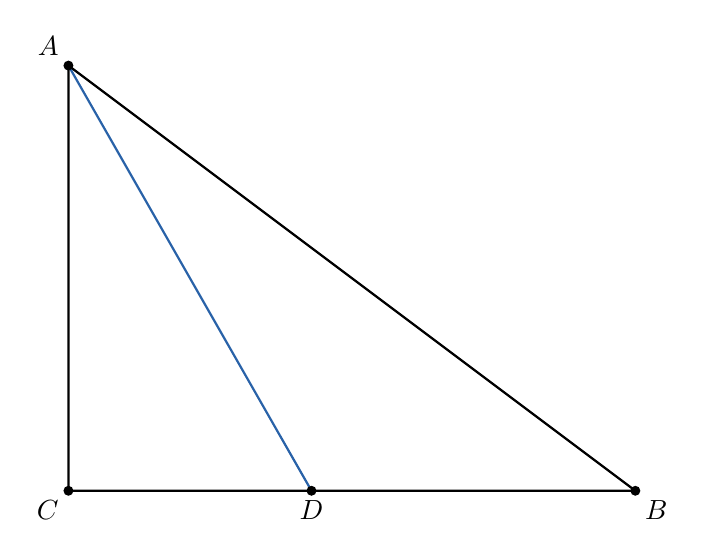
\begin{tikzpicture}[scale=0.9]
  \coordinate (A) at (0, 6);
  \coordinate (B) at (8, 0);
  \coordinate (C) at (0, 0);
  \coordinate (D) at (3.43, 0);
  \draw[thick] (A)--(B)--(C)--cycle;
  \draw[thick, mainblue] (A)--(D);
  \fill (A) circle (2pt) node[above left] {\(A\)};
  \fill (B) circle (2pt) node[below right] {\(B\)};
  \fill (C) circle (2pt) node[below left] {\(C\)};
  \fill (D) circle (2pt) node[below] {\(D\)};
\end{tikzpicture}
\end{center}

利用角平分线性质，作 \(DE \perp AB\) 于 \(E\)。

\(\because AD\) 平分 \(\angle BAC\)，\(\therefore DC = DE\)（到两边距离相等）。

在 \(Rt\triangle ABC\) 中，\(AB = \sqrt{6^2 + 8^2} = 10\)。

由角平分线定理：\(\dfrac{BD}{DC} = \dfrac{AB}{AC} = \dfrac{10}{6} = \dfrac{5}{3}\)。

\(\therefore BD = \dfrac{5}{8} \times 8 = 5\)，\(DC = 3\)。

\(\therefore DE = DC = 3\)。

\[S_{\triangle ABD} = \frac{1}{2} \cdot AB \cdot DE = \frac{1}{2} \times 10 \times 3 = 15\]

\(\therefore \triangle ABD\) 的面积为 \(15\)。\hfill\(\square\)

\begin{tipbox}[方法总结]
\textbf{对称/翻折法}的精髓：利用对称将分散的线段集中，或将折线化为直线。角平分线天然就是一条对称轴——作关于角平分线的对称点，往往能快速转移线段和角度。将军饮马问题是对称法最经典的应用。
\end{tipbox}

% ============================================================
%  技巧八：面积法
% ============================================================
\section*{\textcolor{mainblue}{技巧八：面积法}}

\begin{knowledgebox}[什么是面积法？]
\textbf{核心原理：}同一个图形的面积可以用不同的方式表示。通过建立面积等式，可以得到线段之间的关系，而无需直接计算线段长度。

\medskip
\noindent\textbf{两种常用模式：}

\textbf{模式一：同一面积，不同底和高}

\(S_{\triangle ABC} = \dfrac{1}{2} \cdot a \cdot h_a = \dfrac{1}{2} \cdot b \cdot h_b = \dfrac{1}{2} \cdot c \cdot h_c\)

\textbf{模式二：整体面积 = 部分面积之和}

\(S_{\triangle ABC} = S_{\triangle ABD} + S_{\triangle ACD}\)

\medskip
\noindent\textbf{适用场景：}
\begin{itemize}[leftmargin=1.5em]
  \item 需要求线段的\textbf{比例}或\textbf{长度}；
  \item 有\textbf{高}或\textbf{垂线}条件；
  \item 角平分线条件（配合到两边距离相等）；
  \item 用面积比代替线段比。
\end{itemize}
\end{knowledgebox}

% --- 例题 8-1 ---
\begin{examplebox}[【例题 8-1】同一面积不同表示]
\textbf{已知：}如图，在 \(\triangle ABC\) 中，\(AB = AC = 5\)，\(BC = 6\)。

\textbf{求：}\(\triangle ABC\) 的面积。
\end{examplebox}

\noindent\textbf{解：}

\begin{center}
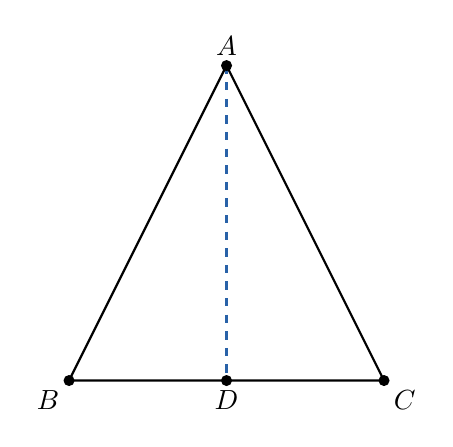
\begin{tikzpicture}[scale=1.0]
  \coordinate (A) at (2, 4);
  \coordinate (B) at (0, 0);
  \coordinate (C) at (4, 0);
  \coordinate (D) at (2, 0);
  \draw[thick] (A)--(B)--(C)--cycle;
  \draw[thick, dashed, mainblue] (A)--(D);
  \fill (A) circle (2pt) node[above] {\(A\)};
  \fill (B) circle (2pt) node[below left] {\(B\)};
  \fill (C) circle (2pt) node[below right] {\(C\)};
  \fill (D) circle (2pt) node[below] {\(D\)};
\end{tikzpicture}
\end{center}

作 \(AD \perp BC\) 于 \(D\)。

\(\because AB = AC\)，\(\therefore D\) 为 \(BC\) 的中点，\(BD = 3\)。

在 \(Rt\triangle ABD\) 中，\(AD = \sqrt{AB^2 - BD^2} = \sqrt{25 - 9} = 4\)。

\[S_{\triangle ABC} = \frac{1}{2} \cdot BC \cdot AD = \frac{1}{2} \times 6 \times 4 = 12\]

\hfill\(\square\)

\begin{tipbox}[思路点拨]
等腰三角形中，作底边上的高是基本操作。求面积时，选择合适的"底"和"高"是关键。面积法不仅用于求面积本身，更是建立线段关系的有力工具。
\end{tipbox}

% --- 例题 8-2 ---
\begin{examplebox}[【例题 8-2】面积法证比例——等积变换]
\textbf{已知：}如图，在 \(\triangle ABC\) 中，\(D\) 在 \(BC\) 上，\(AD\) 与 \(BE\) 交于 \(P\)。

\textbf{求证：}\(\dfrac{BD}{DC} = \dfrac{S_{\triangle ABD}}{S_{\triangle ACD}}\)，并由此推出 \(\dfrac{BD}{DC} = \dfrac{S_{\triangle BPD}}{S_{\triangle CPD}}\)。
\end{examplebox}

\noindent\textbf{证明：}

\begin{center}
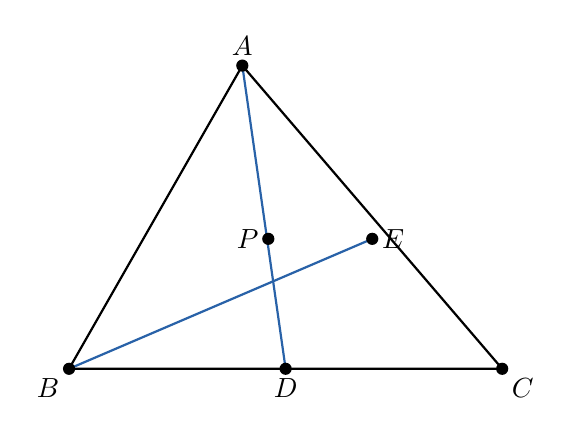
\begin{tikzpicture}[scale=1.1]
  \coordinate (A) at (2, 3.5);
  \coordinate (B) at (0, 0);
  \coordinate (C) at (5, 0);
  \coordinate (D) at (2.5, 0);
  \coordinate (P) at (2.3, 1.5);
  \coordinate (E) at (3.5, 1.5);
  \draw[thick] (A)--(B)--(C)--cycle;
  \draw[thick, mainblue] (A)--(D);
  \draw[thick, mainblue] (B)--(E);
  \fill (A) circle (2pt) node[above] {\(A\)};
  \fill (B) circle (2pt) node[below left] {\(B\)};
  \fill (C) circle (2pt) node[below right] {\(C\)};
  \fill (D) circle (2pt) node[below] {\(D\)};
  \fill (E) circle (2pt) node[right] {\(E\)};
  \fill (P) circle (2pt) node[left] {\(P\)};
\end{tikzpicture}
\end{center}

过 \(A\) 作 \(AH \perp BC\) 于 \(H\)。

\[S_{\triangle ABD} = \frac{1}{2} \cdot BD \cdot AH, \quad S_{\triangle ACD} = \frac{1}{2} \cdot CD \cdot AH\]

\[\therefore \frac{S_{\triangle ABD}}{S_{\triangle ACD}} = \frac{BD}{CD} = \frac{BD}{DC}\]

对于第二个结论：过 \(P\) 作 \(PK \perp BC\) 于 \(K\)。

\[S_{\triangle BPD} = \frac{1}{2} \cdot BD \cdot PK, \quad S_{\triangle CPD} = \frac{1}{2} \cdot CD \cdot PK\]

\[\therefore \frac{S_{\triangle BPD}}{S_{\triangle CPD}} = \frac{BD}{DC}\]

\hfill\(\square\)

\medskip
\textbf{应用举例：}若已知 \(BD:DC = 3:2\)，\(S_{\triangle ABC} = 20\)，则：

\[S_{\triangle ABD} = \frac{3}{5} \times 20 = 12, \quad S_{\triangle ACD} = \frac{2}{5} \times 20 = 8\]

\begin{tipbox}[方法总结]
\textbf{面积法}的核心思想：\textbf{同一个三角形，用不同的底和高表示面积}，由此建立线段的比例关系。面积法特别适合以下场景：
\begin{itemize}[leftmargin=1.5em]
  \item 有公共高的两个三角形，面积比 = 底边比；
  \item 有公共底的两个三角形，面积比 = 高的比；
  \item 角平分线条件 + 面积法 = 求线段长（如技巧三例题 3-2）。
\end{itemize}
面积法的威力在于：不需要计算具体的角度或长度，只需用面积等式即可建立关系。
\end{tipbox}

% ============================================================
%  综合练习
% ============================================================
\newpage
\section*{\textcolor{mainblue}{综合练习}}

\noindent 以下 8 道题分别对应八大技巧，请独立完成后对照参考答案。

\begin{exerbox}[【第 1 题】倍长中线法]
在 \(\triangle ABC\) 中，\(M\) 是 \(BC\) 的中点，\(AB = 5\)，\(AC = 7\)。求 \(AM\) 的取值范围。
\end{exerbox}

\begin{exerbox}[【第 2 题】截长补短法]
在 \(\triangle ABC\) 中，\(\angle BAC = 60^\circ\)，\(BD\) 平分 \(\angle ABC\) 交 \(AC\) 于 \(D\)，\(CE\) 平分 \(\angle ACB\) 交 \(AB\) 于 \(E\)，\(BD\) 与 \(CE\) 交于 \(I\)（内心）。求证：\(BC = BE + CD\)。
\end{exerbox}

\begin{exerbox}[【第 3 题】角平分线辅助线]
在 \(\triangle ABC\) 中，\(\angle C = 90^\circ\)，\(AC = 3\)，\(BC = 4\)，\(CD\) 是 \(\angle ACB\) 的平分线。求 \(CD\) 的长。
\end{exerbox}

\begin{exerbox}[【第 4 题】构造中位线]
在 \(\triangle ABC\) 中，\(D\)、\(E\) 分别是 \(AB\)、\(AC\) 的中点，\(F\) 是 \(DE\) 上一点且 \(DF = 2EF\)。连接 \(CF\) 并延长交 \(AB\) 于 \(G\)。求 \(AG:GB\) 的值。
\end{exerbox}

\begin{exerbox}[【第 5 题】作平行线]
在 \(\triangle ABC\) 中，\(D\) 在 \(BC\) 上，\(BD:DC = 3:2\)，\(E\) 在 \(AD\) 上，\(AE:ED = 2:1\)，\(BE\) 延长交 \(AC\) 于 \(F\)。求 \(AF:FC\)。
\end{exerbox}

\begin{exerbox}[【第 6 题】旋转法]
等边 \(\triangle ABC\) 的边长为 2，\(P\) 是 \(\triangle ABC\) 内一点，且 \(\angle BPC = 150^\circ\)，\(PB = 1\)，\(PC = \sqrt{3}\)。求 \(PA\) 的长。
\end{exerbox}

\begin{exerbox}[【第 7 题】对称/翻折法]
点 \(A(0, 4)\) 和点 \(B(6, 2)\) 在 \(x\) 轴的上方，在 \(x\) 轴上找一点 \(P\)，使 \(PA + PB\) 最小。求 \(P\) 的坐标和 \(PA + PB\) 的最小值。
\end{exerbox}

\begin{exerbox}[【第 8 题】面积法]
在 \(\triangle ABC\) 中，\(D\) 在 \(BC\) 上，\(BD:DC = 2:3\)，\(E\) 在 \(AD\) 上，\(AE:ED = 3:1\)。若 \(S_{\triangle ABC} = 40\)，求 \(S_{\triangle BDE}\)。
\end{exerbox}

% ============================================================
%  参考答案
% ============================================================
\subsection*{\textcolor{tipgreen}{参考答案}}

\begin{knowledgebox}[第 1 题 参考答案]
倍长 \(AM\) 至 \(N\)，使 \(MN = AM\)，连接 \(BN\)。则 \(\triangle AMB \cong \triangle NMC\)，\(BN = AC = 7\)。

在 \(\triangle ABN\) 中，\(AB + BN > AN\) 且 \(BN - AB < AN\)：

\(5 + 7 > 2AM \Rightarrow AM < 6\)，

\(7 - 5 < 2AM \Rightarrow AM > 1\)。

\(\therefore 1 < AM < 6\)。
\end{knowledgebox}

\begin{knowledgebox}[第 2 题 参考答案]
在 \(BC\) 上截取 \(BF = BE\)，连接 \(IF\)。\(\because BI\) 平分 \(\angle B\)，\(BE = BF\)，\(BI = BI\)，

\(\therefore \triangle BIE \cong \triangle BIF\)（SAS），\(IE = IF\)。

\(\because \angle BIC = 180^\circ - \dfrac{\angle B + \angle C}{2} = 180^\circ - \dfrac{120^\circ}{2} = 120^\circ\)。

\(\therefore \angle EIF = 180^\circ - \angle BIC = 60^\circ\)（因为 \(\angle BIE = \angle BIF\)，\(\angle EIB + \angle BIF + \angle FIE = 360^\circ\)）。

\(\because IE = IF\)，\(\angle EIF = 60^\circ\)，\(\therefore \triangle IEF\) 为等边三角形，\(EF = IE\)。

类似地，在 \(BC\) 上截取 \(CG = CD\)，连接 \(IG\)，可得 \(\triangle IDG\) 为等边三角形，\(DG = ID\)。

又 \(\angle FIG = 60^\circ\)（由角度计算可得），故 \(F\)、\(E\)、\(G\) 在 \(BC\) 上排列为 \(B\)、\(F\)、\(G\)、\(C\)（或 \(B\)、\(G\)、\(F\)、\(C\)），且 \(FG = EF = IE\)。

\(\therefore BC = BF + FG + GC = BE + CD\)。（这里利用了 \(FG = IE = EF = DG\) 的关系。）

\medskip
\textbf{提示：}此题核心在于利用内心的角度关系 \(\angle BIC = 120^\circ\) 和截长法构造等边三角形。
\end{knowledgebox}

\begin{knowledgebox}[第 3 题 参考答案]
\(AB = \sqrt{3^2 + 4^2} = 5\)。由角平分线定理：\(\dfrac{AD}{DB} = \dfrac{AC}{BC} = \dfrac{3}{4}\)。

\(\therefore AD = \dfrac{15}{7}\)，\(BD = \dfrac{20}{7}\)。

过 \(D\) 作 \(DE \perp AC\) 于 \(E\)。\(\because CD\) 平分 \(\angle ACB\)，\(D\) 到 \(AC\) 和 \(BC\) 的距离相等，设为 \(d\)。

\(S_{\triangle ABC} = S_{\triangle ACD} + S_{\triangle BCD}\)，

\(\dfrac{1}{2} \times 3 \times 4 = \dfrac{1}{2} \times 3 \times d + \dfrac{1}{2} \times 4 \times d = \dfrac{7d}{2}\)。

\(\therefore d = \dfrac{12}{7}\)。

在 \(Rt\triangle CDE\) 中，\(\angle DCE = 45^\circ\)（角平分线平分 \(90^\circ\)），

\(CD = \dfrac{d}{\sin 45^\circ} = \dfrac{12/7}{\sqrt{2}/2} = \dfrac{12\sqrt{2}}{7}\)。

\(\therefore CD = \dfrac{12\sqrt{2}}{7}\)。
\end{knowledgebox}

\begin{knowledgebox}[第 4 题 参考答案]
用坐标法。设 \(A = (0, 0)\)，\(B = (2, 0)\)，\(C = (0, 2)\)。

\(D = (1, 0)\)，\(E = (0, 1)\)。\(F\) 在 \(DE\) 上且 \(DF = 2EF\)：

\(F = D + \dfrac{2}{3}(E - D) = (1, 0) + \dfrac{2}{3}(-1, 1) = \left(\dfrac{1}{3}, \dfrac{2}{3}\right)\)。

\(CF\) 的参数方程：\((0, 2) + t\left(\dfrac{1}{3}, -\dfrac{4}{3}\right)\)。

与 \(AB\)（即 \(y = 0\)）交点：\(2 - \dfrac{4t}{3} = 0\)，\(t = \dfrac{3}{2}\)。

\(G = \left(\dfrac{1}{2}, 0\right)\)。\(\therefore AG = \dfrac{1}{2}\)，\(GB = \dfrac{3}{2}\)。

\(\therefore AG:GB = 1:3\)。
\end{knowledgebox}

\begin{knowledgebox}[第 5 题 参考答案]
过 \(A\) 作 \(AG \parallel BC\) 交 \(BF\) 延长线于 \(G\)。

\(\triangle AEG \sim \triangle DEB\)：\(\dfrac{AG}{BD} = \dfrac{AE}{ED} = 2\)，\(AG = 2BD\)。

\(\triangle AGF \sim \triangle CBF\)：\(\dfrac{AF}{FC} = \dfrac{AG}{BC}\)。

设 \(BC = 5\)，\(BD = 3\)，\(AG = 6\)。\(\dfrac{AF}{FC} = \dfrac{6}{5}\)。

\(\therefore AF:FC = 6:5\)。
\end{knowledgebox}

\begin{knowledgebox}[第 6 题 参考答案]
将 \(\triangle BPC\) 绕 \(B\) 顺时针旋转 \(60^\circ\)，使 \(C \to A\)，设 \(P \to P'\)。

\(\triangle BPP'\) 是等边三角形，\(PP' = PB = 1\)。

\(AP' = CP = \sqrt{3}\)。

\(\because \angle BPC = 150^\circ\)，旋转 \(60^\circ\) 后 \(\angle BPA = 360^\circ - 150^\circ - 60^\circ = 150^\circ\)。

\(\therefore \angle P'PA = 150^\circ - 60^\circ = 90^\circ\)。

在 \(Rt\triangle APP'\) 中，\(PA^2 = AP'^2 + PP'^2 = 3 + 1 = 4\)。

\(\therefore PA = 2\)。
\end{knowledgebox}

\begin{knowledgebox}[第 7 题 参考答案]
作 \(A(0, 4)\) 关于 \(x\) 轴的对称点 \(A'(0, -4)\)。

连接 \(A'B\)，方程：过 \((0, -4)\) 和 \((6, 2)\)，斜率 \(k = \dfrac{6}{6} = 1\)，\(y = x - 4\)。

令 \(y = 0\)，\(x = 4\)。\(\therefore P = (4, 0)\)。

\(PA + PB = A'B = \sqrt{6^2 + 6^2} = 6\sqrt{2}\)。

\(\therefore P = (4, 0)\)，最小值为 \(6\sqrt{2}\)。
\end{knowledgebox}

\begin{knowledgebox}[第 8 题 参考答案]
\(\because BD:DC = 2:3\)，\(\therefore S_{\triangle ABD} = \dfrac{2}{5} \times 40 = 16\)。

\(\because AE:ED = 3:1\)，\(\therefore S_{\triangle BDE} = \dfrac{ED}{AD} \cdot S_{\triangle ABD} = \dfrac{1}{4} \times 16 = 4\)。

\(\therefore S_{\triangle BDE} = 4\)。
\end{knowledgebox}

\vfill
\begin{center}
\small\textcolor{gray}{本讲义仅供教学参考，例题可根据学生水平调整难度。}
\end{center}

\end{document}
